\newpage
\mysection{Heap Data Structure}

When you hear the term \textit{heap} your brain can go one of two ways: \gls{heapmemory} or \gls{heapds}. Early on in your CS career, you lean toward the memory version of a heap, since that is fresh on your brain. You just got through allocating dynamic memory with the "new" operator. Where does dynamic memory get stored? Well, the heap! However, this section is about a \gls{heapmemory} that allows for easy implementation of an efficient \gls{prioqueue}\supcite{Heapdata,Priority36}. So, are you wondering why we have a type of memory called "the heap" and a data structure call "a heap"? You aren't the only one. Donald Knuth said that back in 1975, several authors began to call the pool of available memory (not allocated to your process) a "heap"\supcite{knuth1997art}, but he never really clarified who or why. There are other "guesses" but it's not really clear. My opinion is that since "heap" has multiple meanings, it might just fit both scenarios.\\

\textbf{Heap Defintion:}
\begin{itemize}
	\tightlist
	\item n.	A group of things placed or thrown, one on top of the other.
	\item n.	A great deal; a lot.
\end{itemize}

A heap data structure is a group of items, placed one on top of another (with a special order to them), and heap memory could also refer to how the memory is allocated, OR to the excess memory not assigned to any process. Who knows?!? It's a conundrum.\\

This section will discuss the data structure variety that implements a priority queue. More specifically, we will describe an array based implementation of a binary heap. Because of how heap operations work, using an array to store values works. Even though it is possible to store a binary tree in an array, it doesn't mean that we should do it unless certain properties are maintained. If these properties are not maintained, its a sketchy situation at best. Meaning, lots of wasted space and empty slots. See section \hyperlink{abbst}{Array Based Binary Search Trees} for information on how to store a binary search tree in an array. 

\mysubsection{Array Based Binary Heap}

Knowing how to store values in an array as a binary search tree requires the programmer to implement certain algorithms. Likewise, to turn that array based binary tree into a binary heap, we must alter the algorithm (or operations) on how we interact with the data structure. It's the specific algorithms that we apply to generic containers (like an array) that makes them what they are. In the next section, we will take our simple binary search tree algorithm to another level when we add the functionality to implement a binary heap.\\

\mysubsubsection{Background}

A binary heap is a heap data structure that takes the form of a binary tree. The binary heap was introduced by J. W. J. Williams in 1964, as a data structure for  \gls{heapsort}\supcite{Binaryhe5}. It turns out, it could be used for more than sorting values. In fact heaps are a very good way of implementing \textbf{priority queues}'s. All we have to do with our binary tree to make it a heap is make sure that it fulfills the following properties:

\begin{enumerate}
	\tightlist
	\item It stays a \gls{complete} binary tree. 
	\item Each value stored in the tree is either less than or equal (Min Heap) or greater than or equal (Max Heap) to its parent. 
	\item If a child does not meet the previous property, it will be swapped with its parent.
\end{enumerate}

A heap data structure uses multiple methods to maintain its heap structure:

\begin{itemize}
	\tightlist
	\item Insert
	\item Remove 
	\item Heapify
	\item BubbleUp
	\item BubbleDown
\end{itemize}

\mysubsubsection{Overview}

In order to make our heap work efficiently, we will take advantage of the logarithmic nature of the binary tree to represent our heap. In order to guarantee logarithmic performance, we must keep our tree balanced\footnote{Go see the binary tree section for info about logarithmic performance.}. A tree is balanced if the difference of the left and right subtrees differ by no more than 1. We determine if the entire tree is balanced by looking at the height difference from the root's left and right subtrees.\\

We already mentioned we want our heap implementation to be a \gls{complete} binary tree. This means each level has all of its nodes. The exception to this is the bottom level of the tree, which we fill in from left to right. The Figure below shows an example of a complete binary tree with its array implementation.


\begin{figure}[h!]
	\centering
	\begin{subfigure}[b]{0.45\textwidth}
		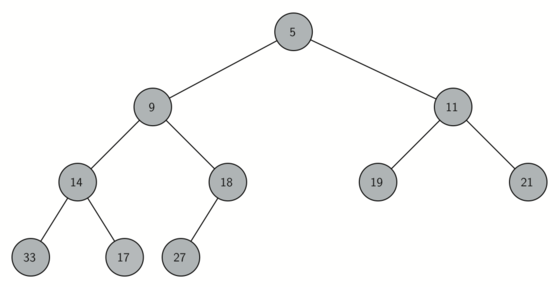
\includegraphics[width=\textwidth]{images/compTree_3013_2020.png}
		\caption{A Complete Binary Tree}
		\label{fig:compbintree}
	\end{subfigure}\\
	\vspace{.5cm}
	\begin{subfigure}[b]{0.45\textwidth}
		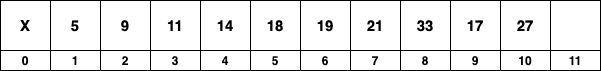
\includegraphics[width=\textwidth]{images/heap_array.png}
		\caption{Array Representation}
		\label{fig:arraytreerep}
	\end{subfigure}
	~ %add desired spacing between images, e. g. ~, \quad, \qquad, \hfill etc. 
	%(or a blank line to force the subfigure onto a new line)
	\caption{A Complete Tree and its Array Representation}\label{fig:arraybintreerep}
\end{figure}


How do we ensure that our heap implementation remains a complete tree? By using the array implementation we discussed above, and inserting new items into the tree by placing them into the next open element in the array. Look at the figure above. By inserting another value at array location 11, we give node 18 a right child, or node 27 a right sibling. Our tree stays "complete". If we were to expand our array and keep inserting into the next available slot, we would continue to fill the tree in from left to right at the bottom, until we started a new row. We never get "holes" in our array, and our tree stays complete and balanced. \\


\mysubsubsection{Heap Operations}

Even though we take advantage of an array based binary tree implementation, it doesn't mean we will insert items the same. In the array based binary tree we would compare our new value to the root of the tree, then find the location to store that value by comparing to the root, and then propagate \textbf{down} the tree moving left and right as needed (see figure \ref{fig:insbintree}).\\

% \begin{center}
% 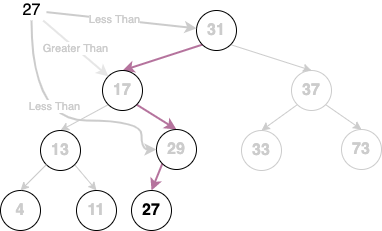
\includegraphics[scale=.45]{images/binary_tree_insert.png} 
% \end{center}

\begin{figure}[h!]
	\centering
	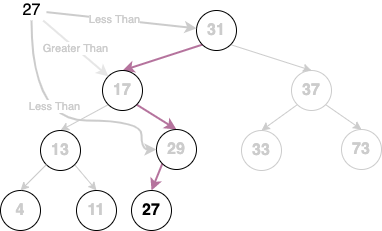
\includegraphics[width=.45\textwidth]{images/binary_tree_insert.png}
	\caption{Inserting into Binary Search Tree}
	\label{fig:insbintree}
\end{figure}

Because the heap property doesn't care about a total ordering of the tree, it only cares about the relationship between parent and child, we can insert values a little differently.\\

\mysubsubsubsection{Insert}

The easiest, and most efficient, way to add an item to a heap is to simply append the item to the next available slot in the array. The good news about this is that it will ALWAYS result in a complete tree. The bad news about appending is that we will very likely violate the heap structure property and have to re-arrange values based on whether it is a min-heap or a max-heap.\\


% \begin{SCfigure}
%     \centering
%     \begin{subfigure}[b]{0.45\textwidth}
%         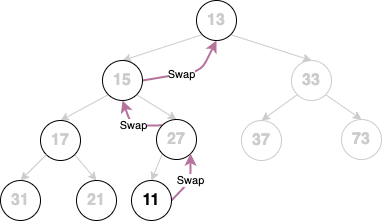
\includegraphics[width=\textwidth]{images/binary_heap_insert.png}
%         \caption{Bubbling Up}
%         \label{fig:heapinsert}
%     \end{subfigure}
%     \begin{subfigure}[b]{0.45\textwidth}
%         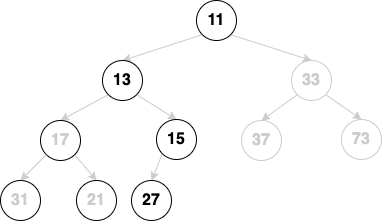
\includegraphics[width=\textwidth]{images/binary_heap_insert_2.png}
%         \caption{After Swaps}
%         \label{fig:heapresult}
%     \end{subfigure}
%     \caption{Inserting value into a heap}\label{fig:heapstuff}
% \end{SCfigure}

\begin{figure}[h!]
	\centering
	\begin{subfigure}[b]{0.45\textwidth}
		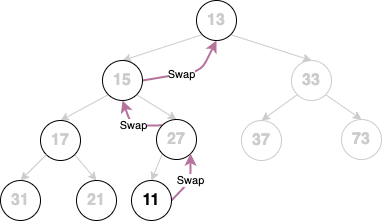
\includegraphics[width=\textwidth]{images/binary_heap_insert.png}
		\caption{Bubbling Up}
		\label{fig:heapinsert}
	\end{subfigure}
	\begin{subfigure}[b]{0.45\textwidth}
		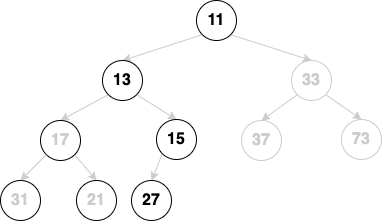
\includegraphics[width=\textwidth]{images/binary_heap_insert_2.png}
		\caption{After Swaps}
		\label{fig:heapresult}
	\end{subfigure}
	\caption{Inserting value into a heap}\label{fig:heapstuff1}
\end{figure}

% \begin{minipage}{0.45\textwidth}
% \begin{figure}
%     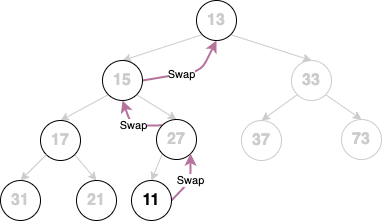
\includegraphics[scale=.33]{images/binary_heap_insert.png}
%     \caption{ Heap Insert Bubble Up}
%     \label{fig:heapex1}
% \end{figure}
% \end{minipage}%
% \hfill%
% \begin{minipage}{0.45\textwidth}
%     \begin{figure}
%     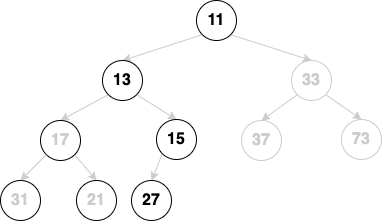
\includegraphics[scale=.33]{images/binary_heap_insert_2.png}
%     \caption{Heap Bubble Up Result}
%     \label{fig:heapex2} 
%     \end{figure}
% \end{minipage}\\

% \begin{center}
% \begin{tabular}{|M{0.40\textwidth}|M{0.40\textwidth}|}
% \hline
% Heap Insert  & Heap Result  \\
% \hline
%   \begin{minipage}[t]{0.40\textwidth}
%     % \vspace{-2ex}

%   \end{minipage}
%  &
%   \begin{minipage}[t]{0.40\textwidth}
%     % \vspace{-2ex}

%   \end{minipage}\\
% \hline
% 11 gets placed at next available location in complete tree, and swaps its way up.&
% Resulting heap after all swaps made. \\
% \hline
% \end{tabular}
% \end{center}


Fixing any violations of the heap structure property can be done by comparing the newly added item with its parent. If the newly added item is less than its parent (assuming a min heap), then we can swap the item with its parent. Since the tree is always a complete tree and therefore balanced, we can assume worse case that an insert item will have to swap \texttt{O(lg n)} times. \\

In \textbf{figure \ref{fig:heapstuff1}} we see an example showing the series of swaps needed to percolate the newly added item up to its proper position in the tree. In table \ref{tab:exinsertheap} we can see the steps (using different values) broken down better.

\begin{center}
	\begin{table}
		\begin{tabular}{|p{0.20\textwidth}|M{0.4\textwidth}|M{0.30\textwidth}|}
			\hline
			  & Array & Binary Tree \\
			\hline
			Append to last slot. &
			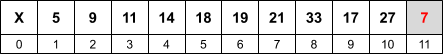
\includegraphics[width=0.4\textwidth]{images/3013_heap_insert_1_2020.png}
			&
			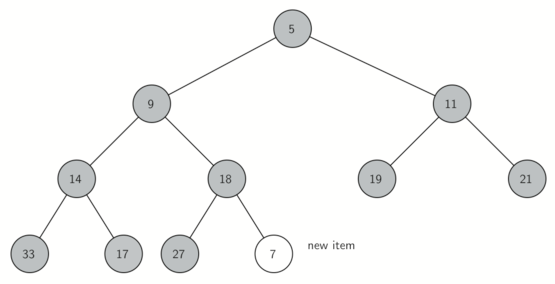
\includegraphics[width=0.25\textwidth]{images/3013_heap_percup_1.png}\\
			\hline
			Swap with smaller parent. &
			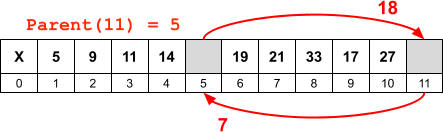
\includegraphics[width=0.4\textwidth]{images/3013_heap_insert_2_2020.png}
			&
			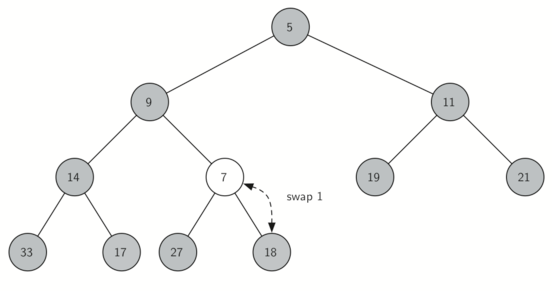
\includegraphics[width=0.25\textwidth]{images/3013_heap_percup_2.png}\\
			\hline
			Swap with smaller parent (again). &
			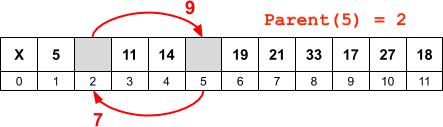
\includegraphics[width=0.4\textwidth]{images/3013_heap_insert_3_2020.png}
			&
			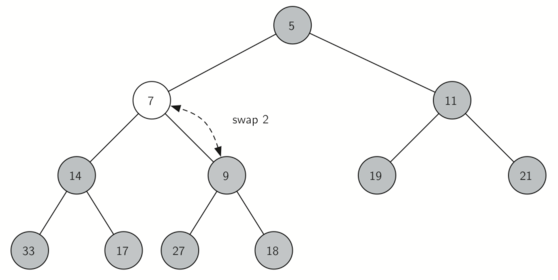
\includegraphics[width=0.25\textwidth]{images/3013_heap_percup_3.png}\\
			\hline
		\end{tabular}
		\caption{Example insert showing comparisons while bubbling up.}
		\label{tab:exinsertheap}
	\end{table}
\end{center}

Notice that when we percolate an item up, we are restoring the heap property between the newly added item and the parent. We are also preserving the heap property for any siblings. Of course, if the newly added item is very small, we may still need to swap it up another level. In fact, we may need to keep swapping until we get to the top of the tree. \textbf{Figure \ref{fig:heapstuff1}} shows the \texttt{Bubble UP} or (percUp, siftUp, etc.) method, which swaps a new item as far up in the tree as it needs to go to maintain the heap property. Again, we use \textbf{\emph{i / 2}} to find the parent and swap the values if the child is smaller than the parent\footnote{Remember, this is a \textbf{minheap}, for \textbf{maxheap} we swap if child is larger.}.\\

\mysubsubsubsection{RemoveMin}

Since the heap property requires that the root of the tree be the smallest item in the tree, finding the minimum item is easy. The involved part of \texttt{RemoveMin} is restoring full compliance with the heap structure and heap order properties after the root has been removed. Restoring compliance can be solved in two simple steps: 1) A swap, and 2) a Bubble Down. More specifically:



\begin{enumerate}
	\def\labelenumi{\arabic{enumi}.}
	\tightlist
	\item
	      Swap the last item in the heap (from the back) to the top of the heap. 
	\item
	      Bubble this item down to its proper position since it will definitely ruin the heap order. 
\end{enumerate}

% \begin{center}
% \begin{tabular}{|p{0.20\textwidth}|M{0.4\textwidth}|M{0.30\textwidth}|}
% \hline
%  & Array & Binary Tree  \\
% \hline
% Append to last slot. &
% 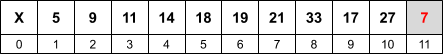
\includegraphics[width=0.4\textwidth]{images/3013_heap_insert_1_2020.png}
% &
% 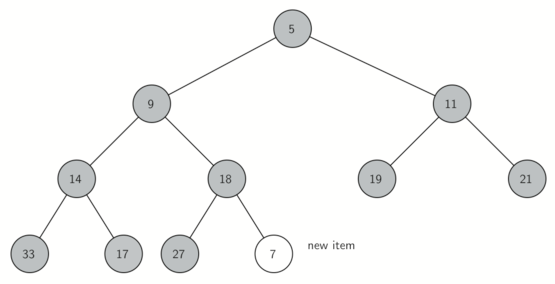
\includegraphics[width=0.25\textwidth]{images/3013_heap_percup_1.png}\\
% \hline

\begin{center}
	\begin{table}
		\begin{tabular}{|p{0.20\textwidth}|M{0.4\textwidth}|M{0.30\textwidth}|}
			\hline
			  & Array & Binary Tree \\
			\hline
			\scriptsize{Remove smallest value (5), swap with last item in array (27).}
			&
			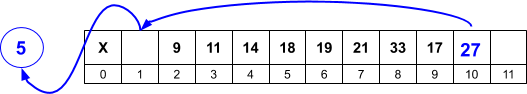
\includegraphics[width=0.40\textwidth]{images/3013_heap_percdown_1_array.png}&
			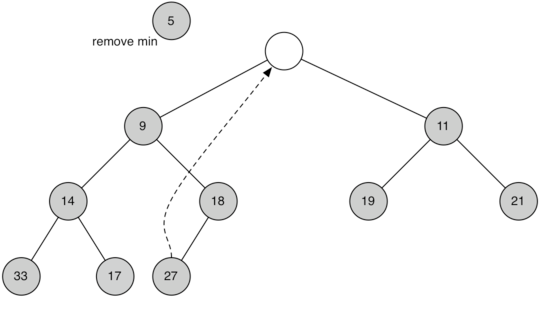
\includegraphics[width=0.30\textwidth]{images/3013_heap_percdown_1.png}\\
			\hline
			\scriptsize{Then start to place the swapped value into it's proper location by comparing it to its children and restoring the heap property.}
			& 
			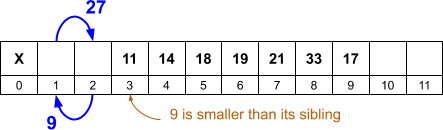
\includegraphics[width=0.40\textwidth]{images/3013_heap_percdown_2_array.png}&
			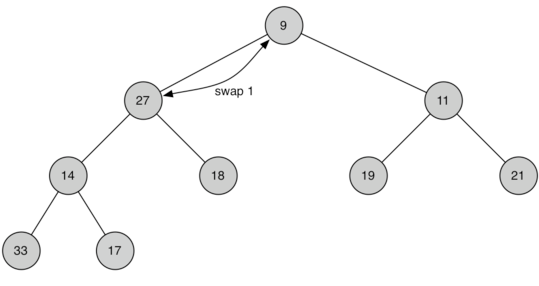
\includegraphics[width=0.30\textwidth]{images/3013_heap_percdown_2.png}\\
			\hline
		\end{tabular}
% 		\caption{Example insert showing comparisons while bubbling up.}
		\label{tab:removemin1}
	\end{table}
\end{center}

\begin{center}
	\begin{table}
		\begin{tabular}{|p{0.20\textwidth}|M{0.4\textwidth}|M{0.30\textwidth}|}
			\hline
			  & Array & Binary Tree \\
			\hline
			\scriptsize{Continue comparing and swapping as long as the heap property is violated (min-heap: parents must be smaller than their children).}
			& 
			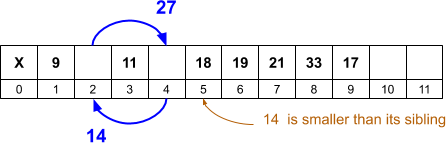
\includegraphics[width=0.40\textwidth]{images/3013_heap_percdown_3_array.png}&
			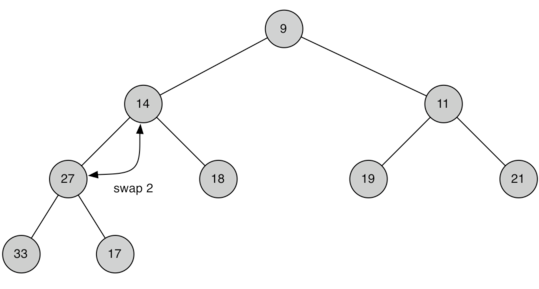
\includegraphics[width=0.30\textwidth]{images/3013_heap_percdown_3.png}\\
			\hline
			\scriptsize{Stop swapping when no child is smaller, or there are no more children to compare to.}
			& 
			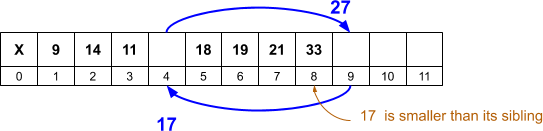
\includegraphics[width=0.40\textwidth]{images/3013_heap_percdown_4_array.png}&
			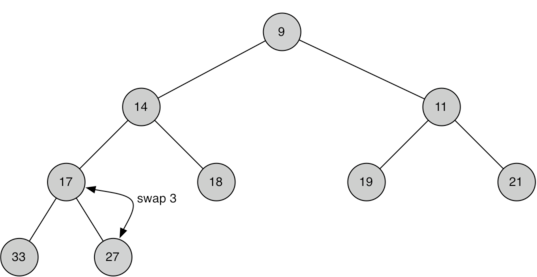
\includegraphics[width=0.30\textwidth]{images/3013_heap_percdown_4.png}\\
			\hline
		\end{tabular}
% 		\caption{Example insert showing comparisons while bubbling up.}
		\label{tab:removemin1}
	\end{table}
\end{center}


\mysubsubsubsection{Heapify}

To finish our discussion of binary heaps, we will look at a method to build an entire heap from an array of keys. If we insert items into the heap, one at a time we would get a performance of \textbf{\textit{O(n lg n)}}. Remember the height of a complete tree is \textbf{\textit{lg n}} (so each new item cannot bubble up further than \textit{lg n}). By inserting \textit{n} items, we get \textbf{\textit{O(n lg n)}} performance. However, if start with an unordered array of keys we can improve that time to 

Inserting n items gives us the first "n". And since we maintain a complete tree, it will be no taller than lg n, and so each can bubble up no further than lg n. 

The first method you might think of may be like the following. Given a list of keys, you could easily build a heap by inserting each key one at a time. Since you are starting with a list of one item, the list is sorted and you could use binary search to find the right position to insert the next key at a cost of approximately \textbf{\emph{O(lg n)}} operations. However, remember that inserting an item in the middle of the list may require \textbf{\emph{O(n)}} operations to shift the rest of the list over to make room for the new key. Therefore, to insert \textbf{\emph{n}} keys into the heap would require a total of \textbf{\emph{O(n lg n)}} operations. However, if we start with an entire list then we can build the whole heap in \textbf{\emph{O(n)}} operations.

\begin{center}
	\begin{table}
		\begin{tabular}{| p{0.25\textwidth}|M{0.30\textwidth}|M{0.35\textwidth}|}
			\hline
			  & Tree Representation & Array Representation \\
			\hline
			\scriptsize{Heapify: Starts with an array of unordered numbers.}
			&
			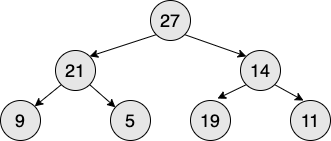
\includegraphics[scale=.30]{images/heapify_tree_01.png}
			&   
			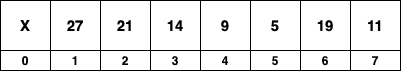
\includegraphics[scale=.30]{images/heapify_01.png}\\
			\hline
		\end{tabular}
		% 		\caption{}
		% 		\label{heap:one}
	\end{table}
\end{center}

\begin{center}
	\begin{table}
		\begin{tabular}{| p{0.25\textwidth}|M{0.30\textwidth}|M{0.35\textwidth}|}
			\hline
			\scriptsize{We can ignore the bottom half of the array since all their children will be off the end of the array.}
			  &   
			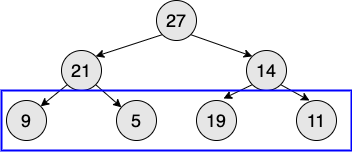
\includegraphics[scale=.30]{images/heapify_tree_02.png}
			  &   
			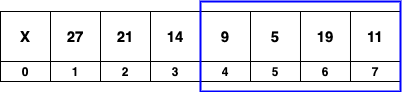
\includegraphics[scale=.30]{images/heapify_02.png}\\
			\hline
		\end{tabular}
	\end{table}
\end{center}

\begin{center}
	\begin{table}
		\begin{tabular}{| p{0.25\textwidth}|M{0.30\textwidth}|M{0.35\textwidth}|}
			\hline
			\scriptsize{Find first location that has 1 or two children, and see if we need to swap (still assume min heap). Index 3 in this table our first candidate.}
			  &   
			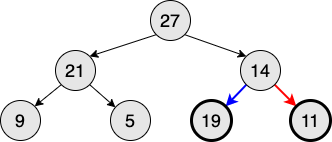
\includegraphics[scale=.30]{images/heapify_tree_03.png}
			  &   
			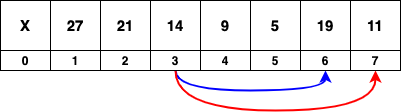
\includegraphics[scale=.30]{images/heapify_03.png}\\
			\hline
		\end{tabular}
	\end{table}
\end{center}


\begin{center}
	\begin{table}
		\begin{tabular}{| p{0.25\textwidth}|M{0.30\textwidth}|M{0.35\textwidth}|}
			\hline
			\scriptsize{Make the swap with the smaller of the two children (11 < 19). 14 cannot bubble down any further so we stop.}
			  &   
			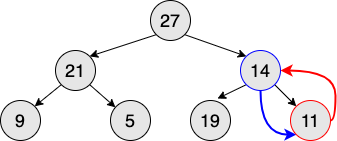
\includegraphics[scale=.30]{images/heapify_tree_04.png}
			  &   
			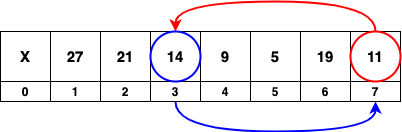
\includegraphics[scale=.30]{images/heapify_04.png}\\
			\hline
		\end{tabular}
	\end{table}
\end{center}


\begin{center}
	\begin{table}
		\begin{tabular}{| p{0.25\textwidth}|M{0.30\textwidth}|M{0.35\textwidth}|}
			\hline
			\scriptsize{We move up one index, and look at our children. Index 2 has children at locations 4 and 5.}
			  &   
			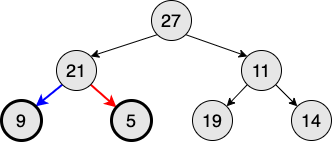
\includegraphics[scale=.30]{images/heapify_tree_05.png}
			  &   
			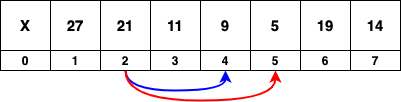
\includegraphics[scale=.30]{images/heapify_05.png}\\
			\hline
		\end{tabular}
	\end{table}
\end{center}


\begin{center}
	\begin{table}
		\begin{tabular}{| p{0.25\textwidth}|M{0.30\textwidth}|M{0.35\textwidth}|}
			\hline
			\scriptsize{We swap index 2 with the smallest of its children (5 < 9). 21 can bubble down no further so we stop.}
			  &   
			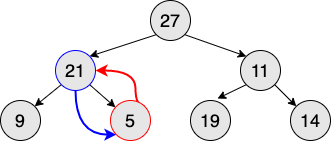
\includegraphics[scale=.30]{images/heapify_tree_06.png}
			  &   
			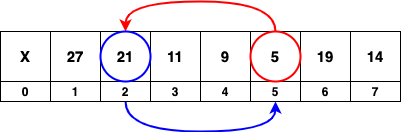
\includegraphics[scale=.30]{images/heapify_06.png}\\
			\hline
		\end{tabular}
	\end{table}
\end{center}


\begin{center}
	\begin{table}
		\begin{tabular}{| p{0.25\textwidth}|M{0.30\textwidth}|M{0.35\textwidth}|}
			\hline
			\scriptsize{We processed indexes 3 then 2 with minimal swapping. We still have index one to process.}
			  &   
			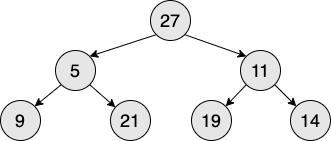
\includegraphics[scale=.30]{images/heapify_tree_07.png}
			  &   
			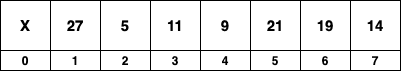
\includegraphics[scale=.30]{images/heapify_07.png}\\
			\hline
		\end{tabular}
	\end{table}
\end{center}


\begin{center}
	\begin{table}
		\begin{tabular}{| p{0.25\textwidth}|M{0.30\textwidth}|M{0.35\textwidth}|}
			\hline
			\scriptsize{We compare index 1 with its two children at indexes 2 and 3. }
			  &   
			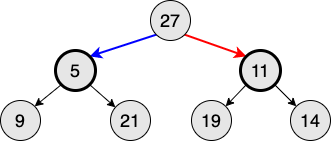
\includegraphics[scale=.30]{images/heapify_tree_08.png}
			  &   
			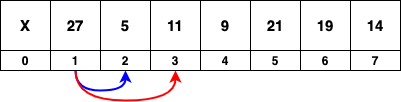
\includegraphics[scale=.30]{images/heapify_08.png}\\
			\hline
		\end{tabular}
	\end{table}
\end{center}


\begin{center}
	\begin{table}
		\begin{tabular}{| p{0.25\textwidth}|M{0.30\textwidth}|M{0.35\textwidth}|}
			\hline
			\scriptsize{We swap index 1 with the smaller of its two children (5 < 11).}
			  &   
			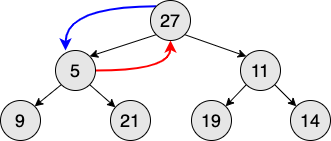
\includegraphics[scale=.30]{images/heapify_tree_09.png}
			  &   
			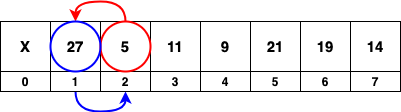
\includegraphics[scale=.30]{images/heapify_09.png}\\
			\hline
		\end{tabular}
	\end{table}
\end{center}


\begin{center}
	\begin{table}
		\begin{tabular}{| p{0.25\textwidth}|M{0.30\textwidth}|M{0.35\textwidth}|}
			\hline
			\scriptsize{The value now at index 2 still has room to bubble down.}
			  &   
			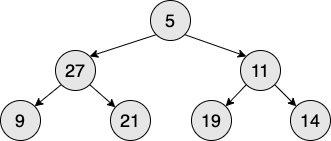
\includegraphics[scale=.30]{images/heapify_tree_10.png}
			  &   
			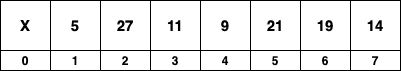
\includegraphics[scale=.30]{images/heapify_10.png}\\
			\hline
		\end{tabular}
	\end{table}
\end{center}


\begin{center}
	\begin{table}
		\begin{tabular}{| p{0.25\textwidth}|M{0.30\textwidth}|M{0.35\textwidth}|}
			\hline
			\scriptsize{We again compare it to its children.}
			  &   
			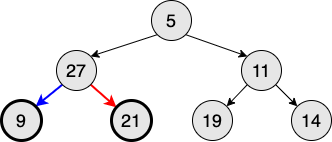
\includegraphics[scale=.30]{images/heapify_tree_11.png}
			  &   
			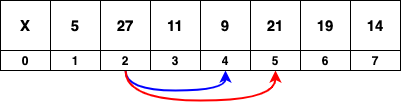
\includegraphics[scale=.30]{images/heapify_11.png}\\
			\hline
		\end{tabular}
	\end{table}
\end{center}


\begin{center}
	\begin{table}
		\begin{tabular}{| p{0.25\textwidth}|M{0.30\textwidth}|M{0.35\textwidth}|}
			\hline
			\scriptsize{The value once again gets swapped with the smaller of its two children. So, this value bubbled down from the 1st index to the bottom of the tree (distance of lg n).} 
			  &   
			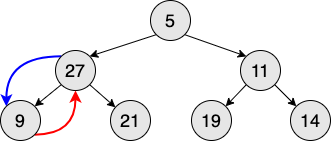
\includegraphics[scale=.30]{images/heapify_tree_12.png}
			  &   
			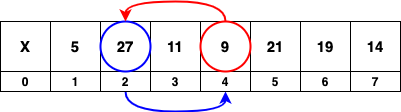
\includegraphics[scale=.30]{images/heapify_12.png}\\
			\hline
		\end{tabular}
	\end{table}
\end{center}


\begin{center}
	\begin{table}
		\begin{tabular}{| p{0.25\textwidth}|M{0.30\textwidth}|M{0.35\textwidth}|}
			\hline
            \scriptsize{We now have a valid min-heap.} 
			  &   
			\includegraphics[scale=.30]{images/heapify_tree_13.png}
			  &   
			\includegraphics[scale=.30]{images/heapify_13.png}\\
			\hline
		\end{tabular}
	\end{table}
\end{center}



% The figure above shows the swaps that the \texttt{Heapify} method makes as it moves the nodes in an initial tree of {[}9, 6, 5, 2, 3{]} into their proper positions. Although we start out in the middle of the tree and work our way back toward the root, the \texttt{percDown} method ensures that the largest child is always moved down the tree. Because the heap is a complete binary tree, any nodes past the halfway point will be leaves and therefore have no children. Notice that when \texttt{i=1}, we are percolating down from the root of the tree, so this may require multiple swaps. As you can see in the bottom most two trees in the figure above, first the 9 is moved out of the root position, but after 9 is moved down one level in the tree, \texttt{percDown} ensures that we check the next set of children farther down in the tree to ensure that it is pushed as low as it can go. In this case it results in a second swap with 3. Now that 9 has been moved to the lowest level of the tree, no further swapping can be done.

The assertion that we can build the heap in \textbf{\emph{O(n)}} may seem a bit mysterious at first, and were not proving anything. However, the key to understanding that you can build the heap in \textbf{\emph{O(n)}} is to remember that the \textbf{\emph{O(lg n)}} factor is derived from the height of the tree. For most of the work in \texttt{Heapify}, the tree is shorter than \textbf{\emph{lg n}}.

Using the fact that you can build a heap from a list in \textbf{\emph{O(n)}} time, you could easily construct a sorting algorithm that uses a heap and sorts a list in \textbf{\emph{O(n lg n)}} cost.